\chapter{An Alternate Approach to Find Continuous Homomorphisms}
\label{chap:alt-hom-approaches}

In this appendix, we describe a technique we attempted to find
continuous homomorphisms. We did not continue, as the approach soon
became intractable.

\section{Modelling the State Space with a Gaussian Process}

We would like to unify our representation of continuous MDPs, using
Gaussian Processes (GP) as standard model; GPs can be easily learnt from
trajectories through the state space, and also model the stochasticity
of the world dynamics. A major limitation of using a Gaussian process to
model action behaviours is uni-modality; only actions which move the
agent in one direction, with noise, can be modelled. This limitation
could be overcome using a mixture of Gaussian processes, but that is out
of the scope of this thesis.

Consider a state space $S$. Let us assume that $S$ is a manifold, with
a mapping into $\Re^n$, $\xi$. For each point $x \in \Re^n$, there is an
associated {\em vector of Gaussian processes}, $\vec{a}$, representing
the behaviour of the actions. The transition dynamics can be described
by the following equation, $$T(s,a,s') = \frac{1}{Z} \exp( (\xi(s')
- m_a(\xi(s)))^T K^{-1}_a(\xi(s)) (\xi(s') - m_a(\xi(s)))),$$ where $m$
and $K$, are the mean and covariance of the Gaussian process. Continuous
actions can also be handled, using $m(\xi(s),\xi(a))$ and
$K^{-1}(\xi(s), \xi(a))$ in place of the respective subscripted
versions.

For the sake of notational convenience, we'll take $S = \Re^n$ in the
sequel. The results we present can be applied to the general continuous
state space through $\xi$.

\begin{figure}[h]
\centering
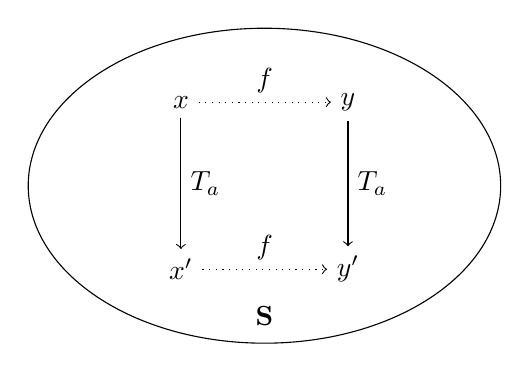
\begin{tikzpicture}
\usetikzlibrary{calc}

% Draw state spaces as rectangles
\draw (0,0) ellipse (3 and 2);
% Draw state space labels
\node at (0,-1.65) {$\mathbf{S}$};

% Xs
\node (x1) at ($(0,0) - (-45:1.5)$) {$x$};
\node (x2) at ($(0,0) - (45:1.5)$) {$x'$};
\draw[->] (x1) to node[auto]{$T_a$}  (x2);

% Ys
\node (y1) at ($(0,0) + (45:1.5)$) {$y$};
\node (y2) at ($(0,0) + (-45:1.5)$) {$y'$};
\draw[->] (y1) to node[auto]{$T_a$}  (y2);

% Map
\draw[->,dotted] (x1) to node[auto]{$f$} (y1);
\draw[->,dotted] (x2) to node[auto]{$f$} (y2);

\end{tikzpicture}
\caption{Bijective Automorphisms}
\label{fig:mdp-hom}
\end{figure}

Now, stating our problem in this framework, we would like to find
bijective automorphisms $f : S \to S$ that preserve the behaviour of the
transition dynamics described by $T_a$ for all actions $a \in \actions$.
At a high level, the diagram \autoref{fig:mdp-hom} describes what we
hope to achieve. Mathematically,
\begin{eqnarray*}
T_a(f(s),f(s')) -  T_a(s,s') &=& 0 \\
\frac{1}{|2\pi K_a(f(s))|} \exp((f(s') - m_a(f(s)))^T K^{-1}_a(f(s)) (f(s') - m_a(f(s)))) &-& \\
 \frac{1}{|2\pi K_a(s)|} \exp((s' - m_a(s))^T K^{-1}_a(s) (s' - m_a(s))) &=& 0.
\end{eqnarray*}

Aside from being in general intractable to solve, the above definition
is too strict for any practical domain. We will now explore two
relaxations that will let us find approximate homomorphisms.

\section{Bayesian Approach}
\label{sec:alt-hom-approaches:bayesian}
In this section, we will consider a Bayesian approach wherein the
mapping $f$ is itself a Gaussian process, $$f(x,y) = \frac{1}{Z}\exp(
(y-n(x))^T L^{-1}(x) (y-n(x)) )$$. We know that the probability of $y$
transitioning to $y'$, given $x$ and $x'$ are the respective pre-images
of $y$ and $y'$, is $T_a(x,x')$; $P(y \to y' | x \to y, x' \to y') = P(x
\to x')$. Thus, we have,

\begin{eqnarray*}
P(y \to y') &=& \int \ud x \ud x' ~ P(y \to y'|x \to y, x' \to y') P(x \to y) P(x' \to y') \\
T_a(y,y') &=& \int \ud x \ud x' ~ T_a(x,x') f(x,y) f(x',y').
\end{eqnarray*}

In the approximate setting, we would like to minimise the KL divergence
between the left and right-hand sides.
\begin{eqnarray*}
  T_a(y,y') &\approx& \int \ud x f(x,y) \E_{x'}[ f(x',y') ].\\
  \mL(y) &=& \E_{y'} [ \log T_a(y,y') - \log \int \ud x f(x,y) \E_{x'}[ f(x',y') ] ].
\end{eqnarray*}

If $\int \ud x f(x,y) = 1$, then we can apply Jensen's inequality to get,
\begin{eqnarray*}
  \mL(y) &\ge& \E_{y'} [ \log T_a(y,y') - \int \ud x f(x,y) \E_{x'}[ \log f(x',y') ] ].
\end{eqnarray*}

Note that $\log f(x',y')$ contains terms of complexity at most $\exp(x^T
A x + b^T x + c)$, which can be evaluated by Gaussian integral.

\begin{note}
  We can also take,
  \begin{eqnarray*}
    \mL(y) &\ge& [ \log T_a(y,y') - \int \ud x f(x,y) \E_{x'}[ \log \E_{y'}[ f(x',y') ] ] ].
  \end{eqnarray*}

  Note that $\E_{y'}$ here is over a {\em different distribution},
  namely $T_a(y,y')$ than $f(x',y')$, and hence not equal to $1$.
\end{note}

To proceed in this direction, we need a prior on $P(x)$, which is hard to
define. More importantly, an implict condition is that $\int \ud x P(x)
f(x,y) = 1$. This involves integrating over the mean function of
a Gaussian process; using the typical Gaussian kernel, the form of the
integrand is $e^{e^{x}}$, which is intractable. 

